\begin{wrapfigure}{l}{0.2\textwidth}
	\begin{center}
	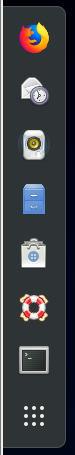
\includegraphics[width=30px]{linuxreader-img018.png}
	\end{center}
	\caption{The Dash}
	\label{fig:de_dash}
\end{wrapfigure}

Aan de linkerkant van je scherm heb je de Dash, ook bekend als de Dock, applicatie bar of taskbar. Als je met je muis over de iconen van de taskbar gaat dan zie je per icoon wat deze betekent. Van boven naar beneden kom je het volgende tegen.

\begin{itemize}
\item Firefox -- een webbrowser
\item Evolution -- Een e-mail client
\item Rhythmbox -- een muziekspeler
\item Files -- Bestandsbrowser
\item Software -- Softwarebeheer
\item Help -- Documentatie
\item Terminal -- Toegang tot de console
\item Show applications -- een beperkt overzicht van beschikbare applicaties.
\end{itemize}

In de volgende hoofdstukken zullen we deze elementen doorlopen maar in een bredere context. We zullen bijvoorbeeld niet alleen Firefox behandelen, maar webbrowsers in zijn algemeenheid.

